% !TeX root = ../main.tex
\section{Sensor Networks and Simplicial Complexes} % (fold)
\label{sec:complexes}

Suppose we would like to learn about the structure of some unknown domain.
Computational techniques are naturally suited to discrete domains, such as a collection of functions on a grid.
One such example is image data in which each image is simply a function on a grid, where each function value is a pixel in the image.
More often the domain in question is not discrete but continuous.
In this case we need some method of discretizing the space in a way that faithfully captures its structure.
This is often achieved by drawing a collection of sample points from the space and studying the relationships between them.
If the sample is representative of the domain and their relationships are induced by a measure on the domain itself we may model the structure of the domain as a graph consisting of vertices for each sample point and edges reflecting their pairwise relationships.

Given an unknown space $\D$ imbued with a metric $\dist:\D\times\D\to\R$ and a set of sample points $P\subset\D$ we may construct a graph with edges between each pair of points within some distance $\e > 0$.
This particular construction is the traditional model for a sensor network in which each node can communicate only with nodes within distance $\e$.
A graph of this network can provide information regarding the connectivity of the nodes, however more information is required if we are interested in the domain itself.

% \begin{figure}[htbp]
%  \centering
%      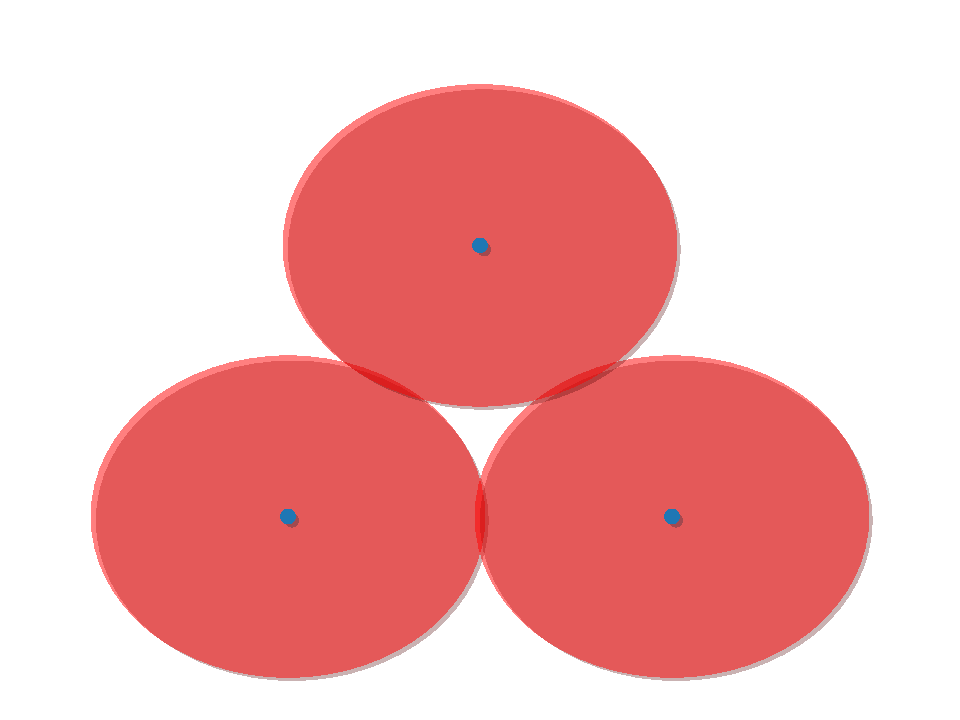
\includegraphics[scale=0.36]{figures/cover1.pdf}
%      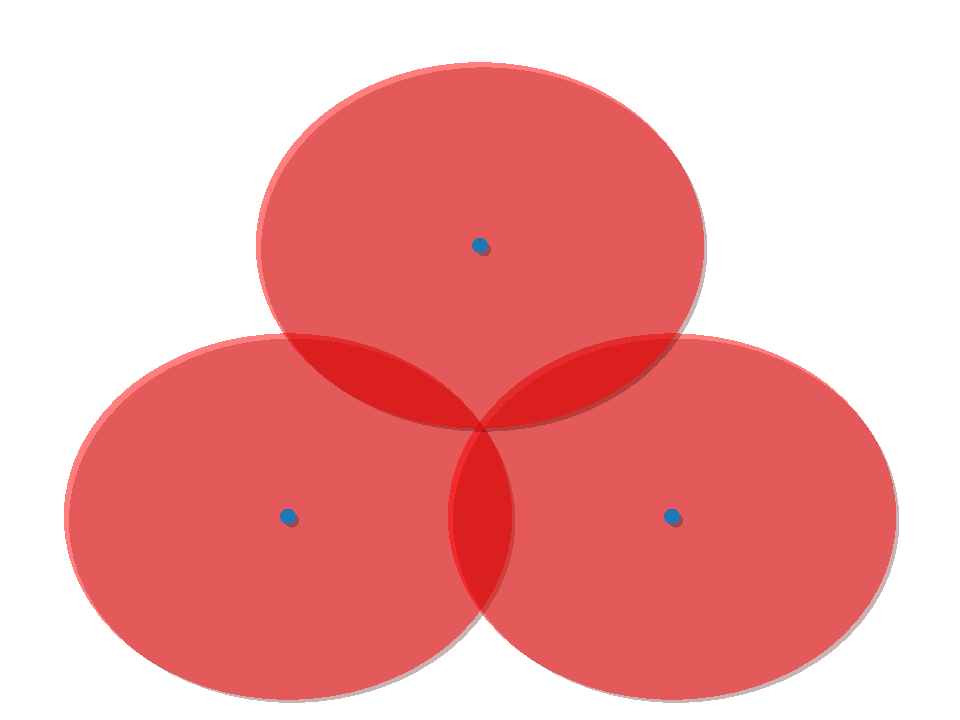
\includegraphics[scale=0.36]{figures/cover2.pdf}
%      \caption{(Left) Coverage regions of three nodes at scale $\e$ with a gap in coverage while each is within pairwise distance $2\e$.
%                 (Right) Coverage regions at scale $\e' > \e$ with coverage.}
%      \label{fig:cover}
%  \end{figure}

Suppose we have a collection of points $P\subset\D$ with \textbf{coverage radius} $\e > 0$.
We define the \textbf{coverage region} of a node $p\in P$ as the set of points in $\D$ within distance $\e$ of $p$, formally
\[ \ball_\e(p) := \{x\in\D\mid \dist(p, x)\leq\e\}, \]
and define the $\e$-offset of $P$, denoted $P^\e$, as
\[ P^\e := \bigcup_{p\in P}\ball_\e(p).\]
A susbet $D\subseteq\D$ is \textbf{covered} by $P$ if $D\subset P^\e$ - each point $x\in D$ is within distance $\e$ of at least one point in $P$.
While a graph is not sufficient for determining if a domain is covered a more robust structure known as a simplicial complex is.
A \textbf{simplicial complex} $K$ is a collection of subsets, called \textbf{simplices}, of a vertex set $V$ that is closed under taking subsets.
That is, for all $\sigma\in K$ and $\tau\subset\sigma$ it must follow that $\tau\in K$.
The \textbf{dimension} of a simplex $\sigma\in K$ is defined as $\dim(\sigma) := |\sigma|-1$ where $|\cdot|$ denotes set cardinality.
The dimension of a simplicial complex $K$ is the maximum dimension of any simplex in $K$.

There is a specific simplicial complex defined for a collection of sets that precisely captures the coverage information we require.
The \textbf{\v Cech complex} of a finite collection of points $P$ at scale $\e > 0$ is defined
\[ \cech^\e(P) := \left\{\sigma \subseteq P\mid \bigcap_{p\in \sigma}\ball_\e(p)\neq \emptyset \right\}. \]
The \v Cech complex is a special case of a more general construction known as a the \textbf{nerve} $\N(\U)$ of a collection of sets $\U = \{U_i\}_{i\in I}$, where $I$ is any indexing set.
The nerve of $\U$ is defined as the simplicial complex with vertex set $I$ such that $\sigma\subseteq I$ is a simplex if and only if \[\bigcap_{i\in \sigma} U_i\neq \emptyset.\]
The collection $\U$ is a \textbf{good cover} if for each $\sigma\subset I$ the set $\bigcap_{i\in\sigma} U_i$ is contractible if it is nonempty.
The \textbf{nerve lemma} states that if $\U$ is a good cover then its nerve $\N(\U)$ is homotopy equivalent to $\bigcup_{i\in I} U_i$.
That is, for a set of nodes $P\subset\D$ such that $\U = \{\ball_\e(p)\mid p\in P\}$ is a good cover the nerve $\N(\U)$ is homotopy equivalent to $P^\e = \bigcup_{p\in P} \ball_\e(p)$.
It follows that the \v Cech complex $\cech_\e(P)$ of $P$ at scale $\e$ is a suitable representation of the coverage region $P^\e$.

\begin{figure}[htbp]
 \centering
     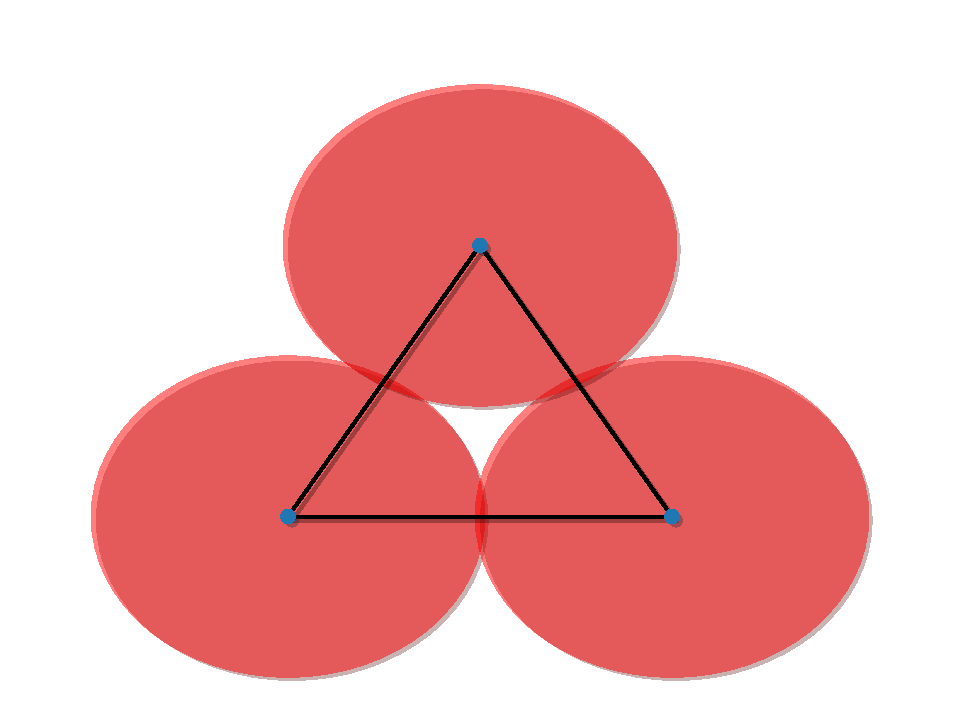
\includegraphics[scale=0.36]{figures/cech1.pdf}
     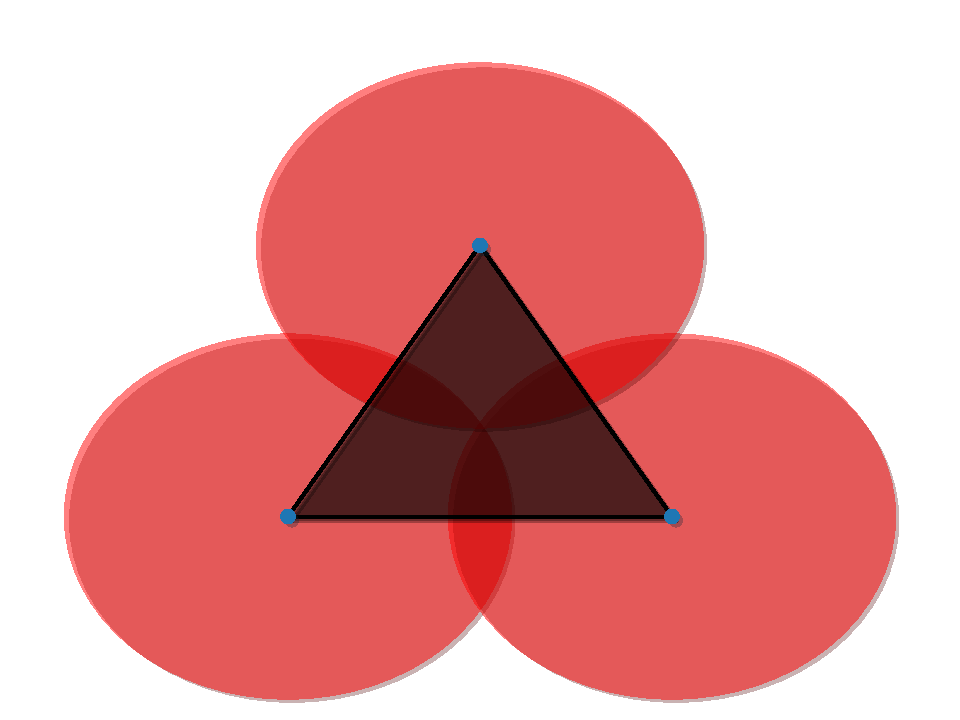
\includegraphics[scale=0.36]{figures/cech2.pdf}
     \caption{\v Cech complexes of three points at scales $\e, \e'$.}
     \label{fig:cech}
 \end{figure}

While the \v Cech complex captures the topology of the coverage region in question exactly it can only be computed when the precise pairwise distances between nodes is known.
If instead we are only provided pairwise \textit{proximity} information indicating when nodes are within some fixed distance we may use the \textbf{(Vietoris-)Rips complex}, defined for a set $P$ at scale $\e > 0$ as
\[ \rips^\e(P) := \left\{\sigma \subseteq P\mid \forall p,q\in\sigma,\ \dist(p, q)\leq\e\right\}. \]

An important result about the relationship of \v Cech and Rips complexes follows from Jung's Theorem~\cite{jung01uber} relating the diameter of a point set $P$ and the radius of the minimum enclosing ball:
\begin{equation}\label{eq:jung_inclusion}
  \cech^\e(P) \subseteq \rips^\e(P) \subseteq \cech^{\jungd \e}(P),
\end{equation}
where the constant $\jungd = \sqrt{\frac{2d}{d+1}}$ (see~\cite{buchet15efficient}).

\begin{figure}[htbp]
 \centering
     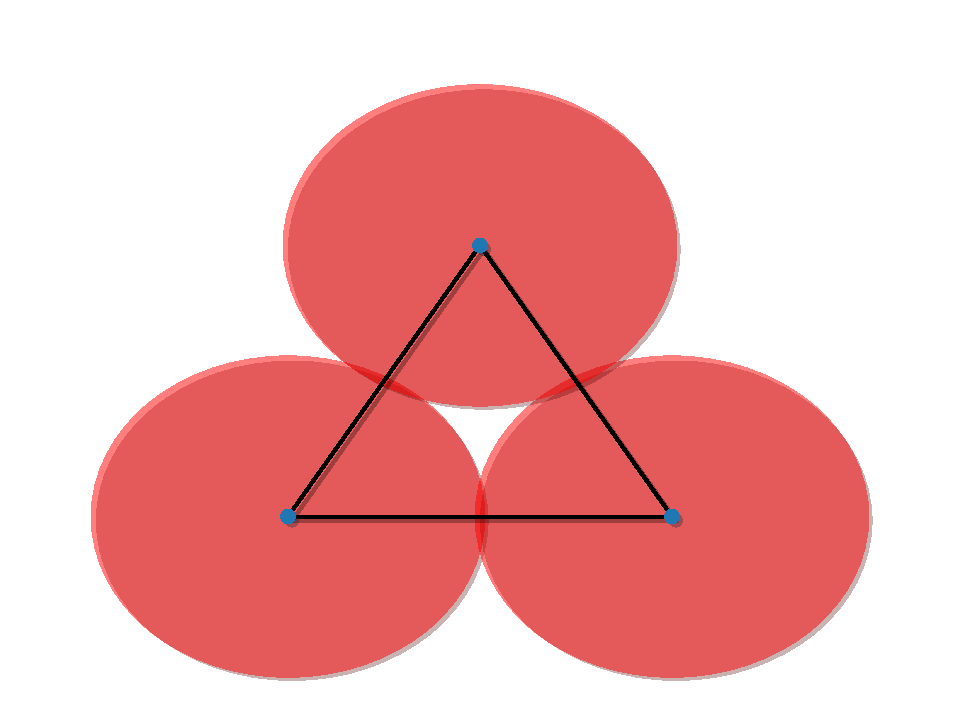
\includegraphics[scale=0.23]{figures/include1.pdf}
     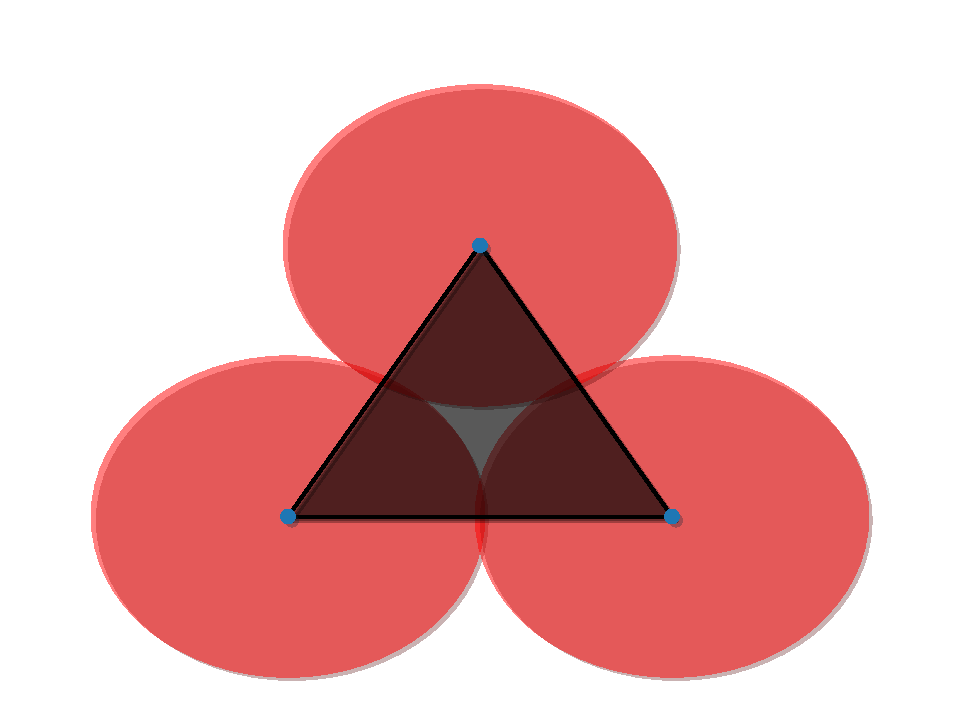
\includegraphics[scale=0.23]{figures/include2.pdf}
     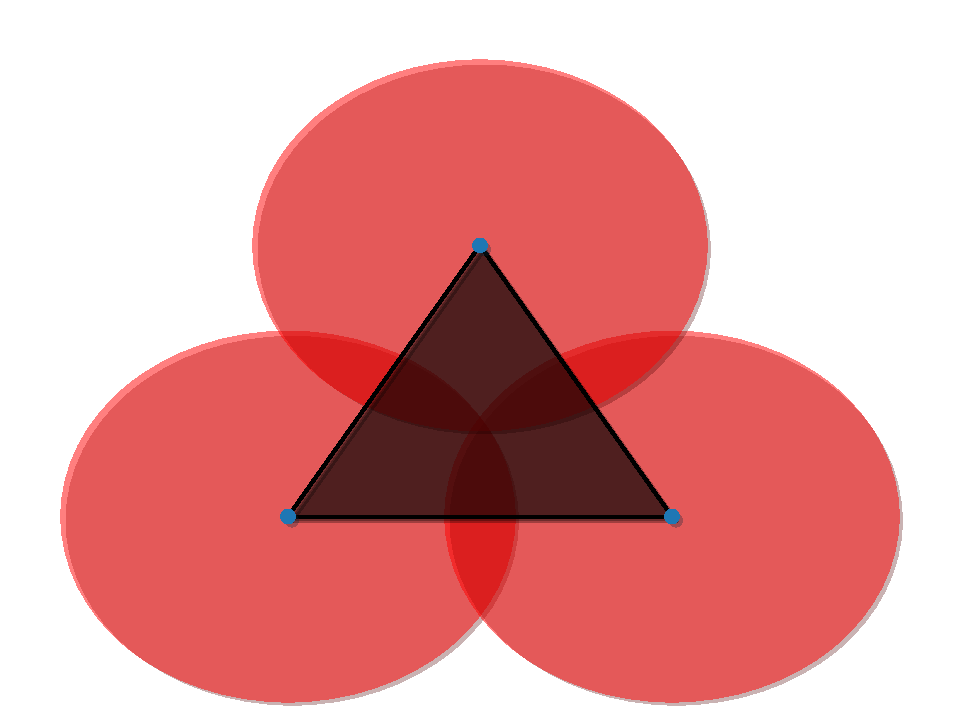
\includegraphics[scale=0.23]{figures/include3.pdf}
     \caption{The Rips-\v Cech interleaving $\cech^\e(P) \subseteq \rips^\e(P) \subseteq \cech^{\jungd \e}(P)$ }
     \label{fig:incluson}
 \end{figure}

As we will see the Rips complex may be used to verify coverage of a domain satisfying some minimal assumptions when we allow the sensors in our network to communicate at two radii $\alpha$ and $\beta$.
In short, if the the inclusion of Rips complexes at scales $\alpha < \beta$ resembles the structure of a subset of the domain then the \v Cech complex at scale $\alpha$, and therefore $P^\alpha$, does as well.

% Sensor networks generally consist of a collection of nodes in some domain with some capacity for communication between them.
% This capability for communication provides local information which can be integrated to reveal global information about the underlying domain.
% Such techniques often rely on knowing the locations of the nodes, which is rarely the case in practice.
% On the other hand, if some minimal assumptions are made about the domain itself we can verify the quality of the network without location information.
%
% We model sensor networks as collections of points sampled from a domain satisfying some minimal assumptions.
% The communication between sensors is represented by a metric on the domain which defines some radius of communication for each node.
% That is, let $\D$ be our domain imbued with some metric $\dist : \D\times\D\to\R$.
% Let $P\subset\D$ be a set of points sampled from $\D$, each representing a node in our sensor network.
% If we assume that each sensor is capable of communicating with nodes within some distance $\alpha > 0$ we may represent the network itself as an undirected graph $G = (P, E)$ with edges for each pair of nodes within distance $\alpha$:
% \[ E = \{(p, q)\in P\mid \dist(p, q)\leq \alpha\}. \]
%
% While this representation does provide some information about the overall connectivity of the network it does not necessarily give us any sense of how well the domain itself is covered.
% That is, if our goal is to determine if every point in a subset $D\subseteq\D$ of the underlying domain is within $\alpha$ of at least one sensor we must verify that $D$ is a subset of the union of the regions spanned by each node's communication radius.
% Formally, let $\ball_\e(p) := \{x\in\D\mid \dist(x, p)\leq\e\}$ denote the coverage region of a node $p\in P$ at radius $\e\in\R$ and \[P^\e := \displaystyle\bigcup_{p\in P}\ball_\e(p)\] denote the region covered by all nodes in $P$, or the $\e$-offset of $P$.
% We say that a subset $D$ of $\D$ is covered by $P$ at radius $\e$ if $D\subseteq P^\e$.
%
% We now define a generalization of a graph which can be used to represent the coverage region of a given sensor network.
% A \textbf{simplicial complex} $K$ is a collection of subsets, called \textbf{simplices}, of a vertex set $V$ that is closed under taking subsets.
% That is, for all $\sigma\in K$ and $\tau\subset\sigma$ it must follow that $\tau\in K$.
% The \textbf{dimension} of a simplex $\sigma\in K$ is defined as $\dim(\sigma) := |\sigma|-1$ where $|\cdot|$ denotes set cardinality.
% The dimension of a simplicial complex $K$ is the maximum dimension of any simplex in $K$.
% We note that an undirected graph $G = (V, E)$ is a 1-dimensional simplicial complex, consisting only of 0-simplices (vertices) $V$ and 1-simplices (edges) $E$.

% \textbf{TODO} simplicial complexes as ways to discretize space.
%
%
% While this information is useful for modeling systems resembing networks with li they are limited by the simplicity of the pairwise information provided.
% If instead relationships between points is given as a measure such as distance or correlation we can impose weights on the edges in order to capture more robust information about the underlying structure.
% Specifically, if are given a collection of points sampled from some domain which induces a measure we can hope to not only model the relationships between points but the structure of underlying space from which they are sampled.
% For example, given an unknown space $\D$ imbued with a metric $\dist:\D\times\D\to\R$ and a collection of points $P\subset\D$ we can use the metric structure imposed on $P$ to build a weighted graph with vertices for each point $p\in P$ and edges $e = (p, q)$ with weights $w_e = \dist(p, q)$.
% If the sample is representative of the underlying domain we would hope that the complete graph consisting of weighted edges for each pair of points in $P$ would capture the structure of the domain itself.
% In practice this representation is not ideal as construction of a complete graph is infeasable due to size of the sample, or some doubt in the quality of the sample.
%
% We are interested in studying some continuous domain which cannot be handled directly, as is often the case in computational problems which operate
% This is often the case in computational problems which operate naturally on discrete domains.

% section complexes (end)
